%Suite géométrique et tableaur

\section{Efficacité d'un antibiotique (7 points)}

Un laboratoire pharmaceutique souhaite tester le temps de réaction d'un nouvel antibiotique contre le bacille de Koch responsable des tuberculoses. Pour cela, on dispose d'une culture de $10^{10}$ bactéries dans laquelle on introduit l'antibiotique. On remarque que le nombre de bactéries est divisé par quatre toutes les heures.

\subsection{\ }

On crée la feuille de calcul suivante donnant le nombre de bactéries en fonction du temps $n$ en heures.

\begin{center}
	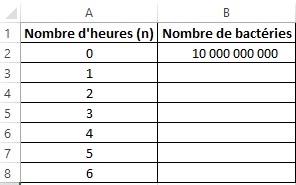
\includegraphics[scale=1]{img/bacteries}
\end{center}

\begin{questions}
	\question[1] Quelle formule faut-il enter dans la cellule \texttt{B3}, pour calculer le nombre de bactéries au bout d'une heure, de sorte qu'en recopiant cette formule vers le bas on puisse compléter les lignes suivantes.
	
	
	\question[1]  On a recopié la formule précédente jusqu'en \texttt{B18} 
		\begin{parts}
			\part[\half] Quelle formule se trouve en \texttt{B18} ?
			\part[\half] Que représente concrètement la valeur calculée dans cette cellule ?
		\end{parts}
	
	
\end{questions}

\subsection{\ }

On note $u_0$ le nombre de bactéries au moment de l'injection de l'antibiotique.
Soit $(u_n)_{n \in \naturels}$, la suite représentant le nombre de bactéries, contenues dans la culture, $n$ heures après l'introduction de l'antibiotique. 

\begin{questions}
	\question[1] Exprimer $u_{n+1}$ en fonction de $u_n$.
	
	\question[1] En déduire que la suite $(u_n)$ est une suite géométrique de raison \num{0.25}.
	
	\question[1] Exprimer $u_n$ en fonction de $n$.
	
	\question[2] Calculer au bout de combien d'heures le nombre de bactéries deviendra inférieur à 100. 
\end{questions}